\section{Confined Compression Test.}
\label{excomp}
We now consider to perform a compression test on a previously swollen slice of ECM, for which the parameters $\chi$ and $G^A_{eq}\equiv G_{vol}$ have been previously estimated with a free swelling experiment. As illustrated in Figure \ref{confcomp}, a porous plate is used so that the fluid is free to flow and the chemical equilibrium with the external bath is restored after the transient relaxation phase. After compression of the tissue in ramps, the system is allowed to relax while the strain $\epsilon$ is maintained constant \cite{Netti}. In this case we are interested in the equilibrium, i.e. relaxed, behaviour. 

\begin{figure}[h]
	\centering
	\def\svgwidth{0.89\linewidth}
	\input{latex/images/compression.pdf_tex}
	\vspace{2mm}
	\caption{Schematic representation of a compression test with a porous piston. A deformation is imposed in the $Z$ direction and the force necessary to maintain the deformation is recorded. }
	\label{confcomp}
\end{figure}

As the deformation is constrained to the $Z$ direction, the tensor $\F$ is of the form:

\begin{equation}
\F=J_0^{1/3}\begin{bmatrix}
1 &0&0\\
0&1&0\\
0&0& \lambda_1
\end{bmatrix},
\label{F} 
\end{equation}
where $\lambda_1 = 1 - \epsilon$ and $J_0=1+v_sC_{s,0}$ defines the initial swollen state for $\lambda_1=1$ . As the problem is one-dimensional, we can reduce the number of unknowns. We define $u=\mathbf{u}\,\cdot\,\mathbf{e}_Z$, $T_{zz}= \mathbf{e}_Z \mathbb{T}\mathbf{e}_Z$ and $J_m=\mathbf{J}_m\,\cdot \,\mathbf{e}_Z$, the component of the displacement, deformation tensor and fluxes in the $Z$ direction. Assuming the slice to have an initial height $H_0$, proper boundary conditions need to be assigned at the two edges $Z=0$ and $Z=H_0$:
\begin{eqnarray}
\left[\mu_s\right]^+_-=\left[\mu_+\right]^+_-=\left[\mu_-\right]^+_-=0, &\qquad& Z=H_0\,,\\
\quad \left[T_{zz}\right]^+_-=0, &\qquad& Z=H_0\,,\\
J_m = u= 0, &\qquad& Z=0\, ,\\
\frac{\d u}{\d Z}=-\epsilon &\qquad& Z=H_0\,,\\
\frac{\d \phi}{\d Z}=0 &\qquad& Z=0,H_0\,.
\end{eqnarray}

At equilibrium, the conditions~1 and 2 listed in Section \ref{free} still hold. On the other hand, due to the external force $\mathbf{F}= -F_z \mathbf{e}_z$ which is exerted on the plate of area $A$, condition 3 now reads:

\begin{equation}
T_{zz}=\sigma = -\frac{F_z}{A}.
\end{equation} 

\subsection{Model Comparison.}
Starting from model A, given the symmetries of the problem, $\B_e$ is a diagonal matrix of the form:
\begin{equation}
\B_e=\begin{bmatrix}
b &0&0\\
0&b&0\\
0&0& b_1
\end{bmatrix}. 
\end{equation}
If we now study the equilibriums of Equation~(\ref{Be}), we obtain that $b=b_1$. Since $\det \B_e= (\det \F)^2$, we conclude that:
\begin{equation}
b = J_0^{2/3}\lambda_1^{2/3}.
\end{equation}

Similarly, we also have that the tensors $\bar{\B}$ and $\bar{\B}_e$ in model B are of the form:
\begin{equation}
\bar{\B}=\begin{bmatrix}
\lambda_1^{-2/3} &0&0\\
0&\lambda_1^{-2/3}&0\\
0&0& \lambda_1^{4/3}
\end{bmatrix}, \qquad
\bar{\B}_e=\begin{bmatrix}
\bar{b} &0&0\\
0&\bar{b}&0\\
0&0& \bar{b}_1
\end{bmatrix}
\end{equation}
with the $\bar{b}=\bar{b}_1=1$ at equilibrium. Consequently, we find that the second spring does not contribute to the stress. Using the boundary condition, we can now compute the pressure and the equilibrium condition:
\begin{gather}
p = \begin{cases}
\displaystyle
-\sigma + \frac{G^A_1}{J_0\lambda_1} (J^{2/3}_0\lambda_1^2-1)+\frac{G^A_2}{J_0\lambda_1} (J_0^{2/3} \lambda_1^{2/3}-1) &\quad \text{MODEL A} \\[10pt]
-\sigma + \dfrac{G_{vol}}{J_0\lambda_1}(J_0^{2/3}\lambda_1^{2/3}-1)+\dfrac{2G^B_1}{3J_0\lambda_1^{5/3}} (\lambda_1^2-1) &\quad \text{MODEL B}
\end{cases}\\[10pt]
\begin{aligned}
\frac{\sigma v_s}{k_B T}=\frac{J_0\lambda_1+\chi}{J_0^2\lambda^2_1}+\frac{pv_s}{k_B T}+&\ln \frac{J_0\lambda_1-1}{J_0\lambda_1} +2c_0v_s\\
-\ &\sqrt{\left(\frac{z_fC_fv_s}{J_0\lambda_1-1}\right)^2+4v_s^2c^2_0}
\end{aligned}\label{compA}
\end{gather}

Unlike the case of unconstrained swelling, we now have that the model $A$ and $B$ are substantially different. There is indeed no choice of parameter values for which the models are equivalent. 

\begin{figure}[h!]
	\begin{subfigure}{0.49\textwidth}
		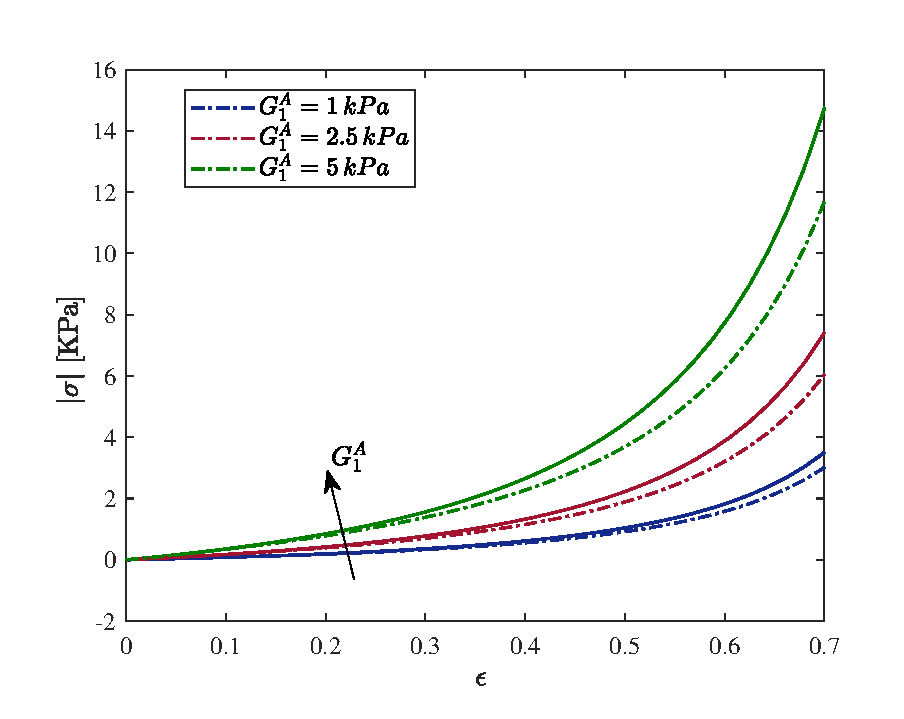
\includegraphics[scale=0.4]{images/comp1}
		\caption{}
	\end{subfigure}
	\begin{subfigure}{0.49\textwidth}
		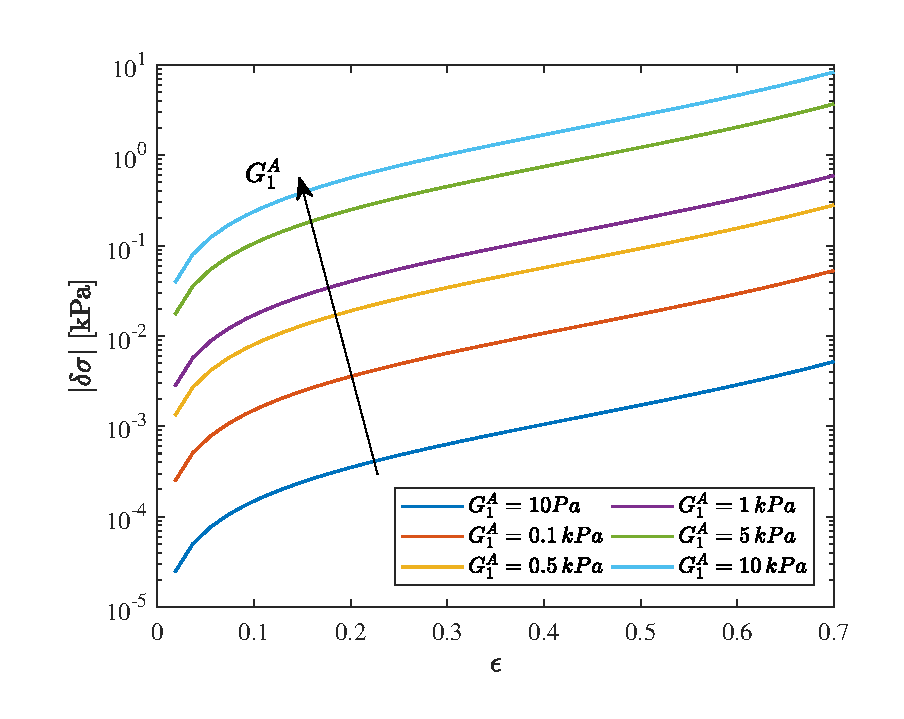
\includegraphics[scale=0.4]{images/comp2}
		\caption{}
	\end{subfigure}
	
	\begin{subfigure}{0.49\textwidth}
		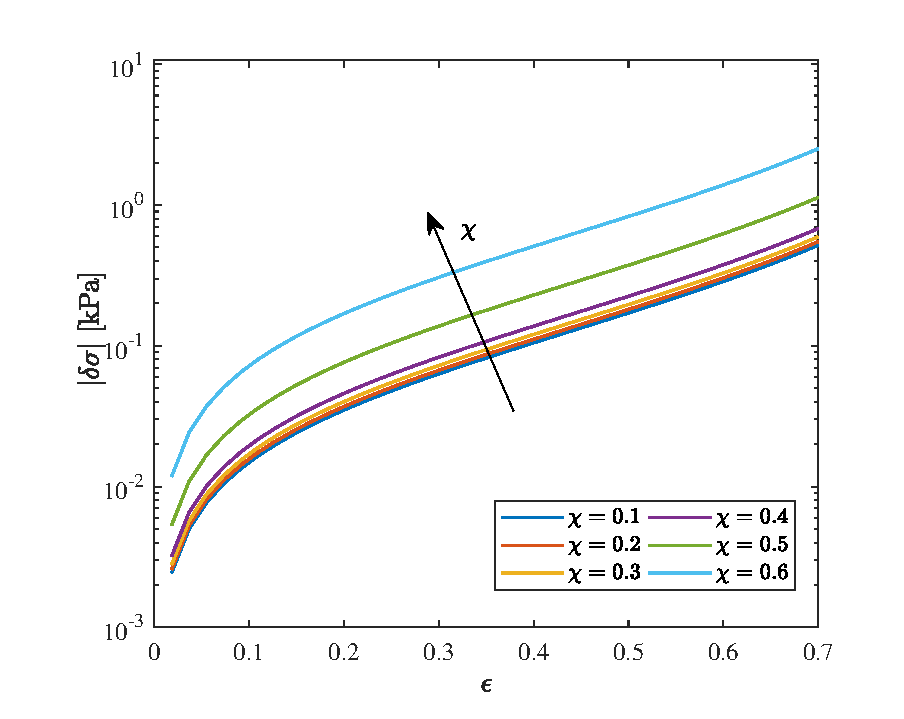
\includegraphics[scale=0.4]{images/comp3}
		\caption{}
	\end{subfigure}
	\begin{subfigure}{0.49\textwidth}
		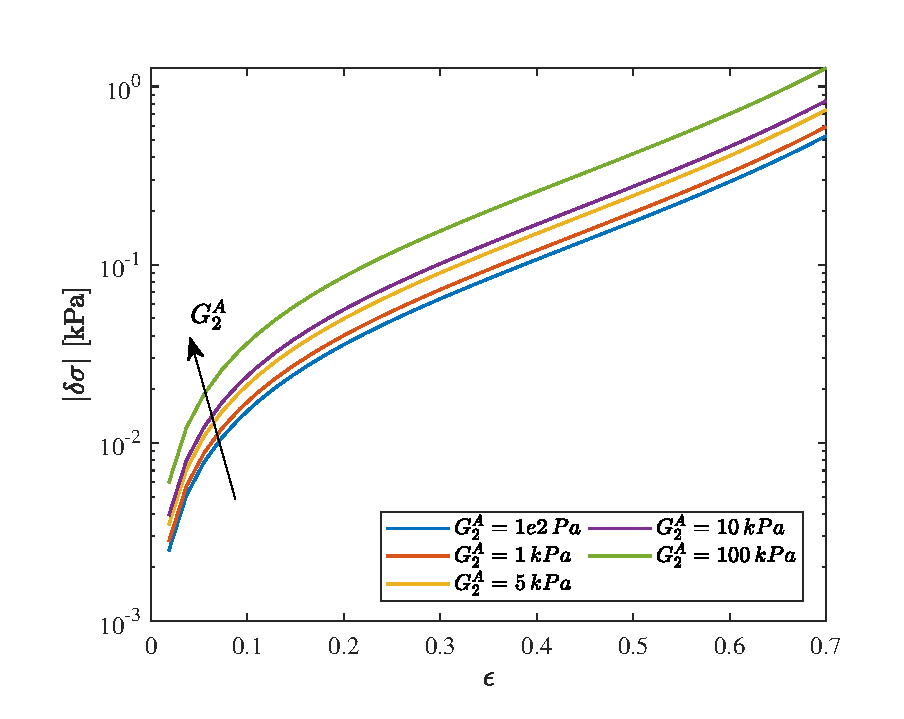
\includegraphics[scale=0.4]{images/comp4}
		\caption{}
	\end{subfigure}
	\caption{Sensitivity Analysis. As expected the mismatch between the two models grows with the strain: (a) Comparison of stress-strain curve predicted by model A (dotted line) and model B (full line) for different values of the parameter $G^A_1$; (b) as $G_1^A$ increases so does the discrepancy $\delta\sigma$; (c) $\delta\sigma$ is also particularly sensitive to changes in the mixing parameter $\chi$, in particular we see that there is a relevant jump when the ECM is in the \textit{collapsed} phase; (d) on the other hand, only large changes in $G^A_2$ have a relevant impact on $\delta\sigma$.}
	\label{comp3}
\end{figure}

As mentioned previously, we first compare the models $A$ and $B$, assuming that the parameters $\chi$ and $G_{vol}=G^A_{eq}$ are fixed so that the equilibrium volume $J_0$ is known. If we now take the difference between the compression stress predicted by the two models, i.e. $\delta \sigma= \sigma_{B}-\sigma_{A}$, we obtain:
\begin{equation}
\delta \sigma = \frac{2 G_1^{B}}{3} \frac{\lambda_1^2-1}{J_0\lambda_1^{5/3}} - \frac{G_1^A}{J_0^{1/3}}(\lambda_1-\lambda_1^{-1/3}).\label{err}
\end{equation}
As there is no constant value of $G^{B}_1$ for which the difference $\delta \sigma$ is identically zero, for the purpose of our analysis, we impose the two models to agree at the second order in the regime of small deformation. This translates in the conditions $\lambda_1\rightarrow 1$:
\begin{equation}
\left.\delta \sigma\right|_{\lambda_1=1}=0 \qquad \left.\frac{\d \delta \sigma}{\d \lambda_1}\right|_{\lambda_1=1}=0 \quad\Rightarrow \quad G_1^{B} = J_0^{2/3}G_1^A.
\end{equation}
Under such conditions we can rewrite Equation~(\ref{err}) as:
\begin{equation}
\delta \sigma(\lambda_1;G^A_1,J_0) = \frac{G_1^A}{J^{1/3}_0\lambda_1^{5/3}} \left(\frac{2}{3}\lambda^2_1-\frac{2}{3}-\lambda_1^{5/3}+\lambda_1^{4/3}\right), 
\end{equation}
which is unbounded for large deformations, i.e. $\lambda_1\rightarrow0$. Note that $J_0$ is implicitly defined by Equation~(\ref{eqF}), where $J_0=\lambda^3$, so that the variation $\delta\sigma$ depends indirectly on all model parameters. As shown in Figure \ref{comp3}, $\chi$ and $G_1^A$ are the two parameters that have impact on $\delta\sigma$ the most. While $G_1^A$ depends only on the properties of the material, $\chi$ can be tuned by changing the temperature $T$ of the experiment. Based on our analysis, we suggest that confined compression experiments can be used to compare the two models and choose the most appropriate. This however when the parameter $\chi$ and $G_{vol}$ are known. 

In real experiment on soft tissue, this is not usually the case. As the slices are naturally swollen, unconstrained swelling experiments are usually not performed and model validation only relies on compression test. However, we suggest that such approach does not provide enough information and can consequently lead to misleading quantitative predictions. As an example, we follow the work of Xue et al. \cite{ecm2}, where the authors validate their poro-hyperelastic model on the data collected by Netti et~al. \cite{Netti} under compression of HSTS 26T sarcoma slices. Fitting both our models to the same data, we show that more rigorous testing is necessary to test constitutive model of soft tissues.
%We here consider another standardd
\subsection{Test on Experimental Data.}
\label{data}
Using the data collected by Netti et~al. \cite{Netti} on HSTS 26T sarcoma slices, we show that the standard compression test is not sufficient on its own to validate a model. Besides the compressive test, Netti et~al. have also measured the composition of the tumour slice, so that the parameters $C_f$ and $c_0$ are known (see Table \ref{Tab1}). The other constant values listed in Table \ref{Tab1} have been taken from the literature. 

Despite our model being built to describe decellularized ECM, cells can be included in the model simply as part of the solid phase \cite{ecm2}. As we are interested in the tissue scale, this is a good approximation. However, as suggested also by Xue et~al.\cite{ecm2}, more accurate models also incorporate the cellular activities. However, this goes beyond the purpose of our study. 

\begin{figure}[h]
	\hspace{-8mm}
	\begin{subfigure}{0.62\textwidth}
		\hspace{2mm}
		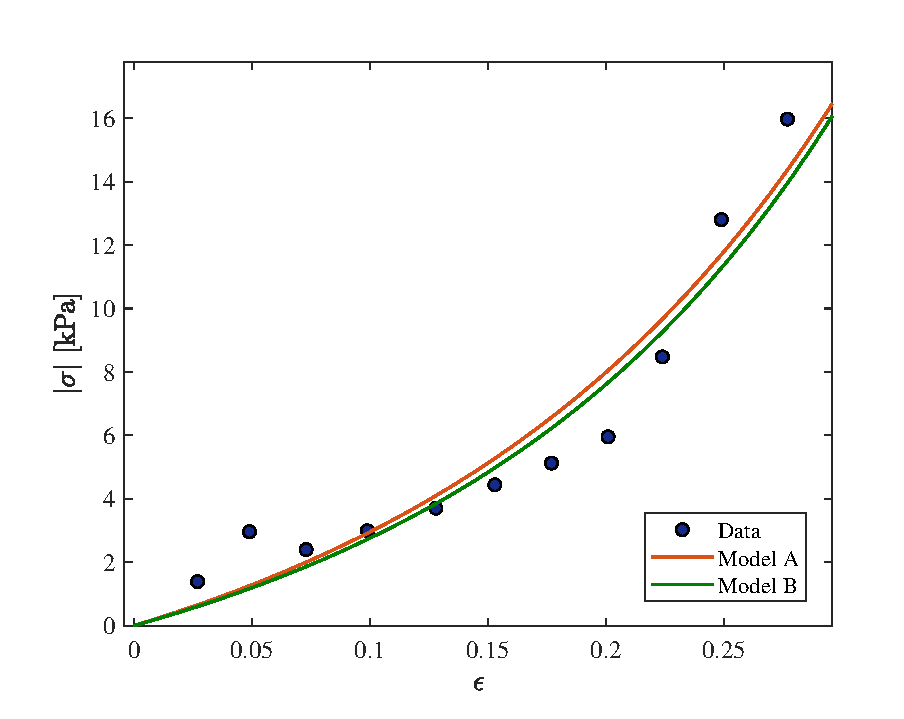
\includegraphics[scale=0.45]{images/compression2.eps}
		\caption{Fitted Model}
		\label{fit}
	\end{subfigure}
	\begin{subtable}{0.375\textwidth}
			\begin{tabular}{c | c ||c| c }		
				\hline\addlinespace[2pt]
				 \multicolumn{2}{c||}{Model A} &  \multicolumn{2}{c}{Model B}\\[0.5mm]
				\hline\addlinespace[2pt]
				$\quad \chi\quad$ & $\quad0.498\quad$ &$\quad \chi\quad$&$\quad0.524\quad$\\[0.5mm]
				$G^A_1$ & 18.9 kPa&$G_{vol}$&75 Pa\\[0.5mm]
				$G^A_2$ & 5.3 Pa&$G^{BA}_{1}$& 55.1 kPa\\[0.5mm]
				$J_0$ & $20.7$&  $J_0$&$14.8$\\[0.5mm]
				\hline
			\end{tabular}
		\caption{Estimated Parameters}
		\label{param}
	\end{subtable}
\caption{Comparison of the two models in fitting real experimental data from \cite{Netti}.}		
\end{figure}

Following \cite{ecm2}, we fit both models to the experimental data, where $C_f$ and $c_0$ are as estimated in \cite{Netti} and the other constants listed in Table \ref{Tab1} have been taken from the literature. Consequently the set of unknown parameters are $\left\{\chi, G^A_1, G^A_2\right\}$ and  $\left\{\chi, G_{vol}, G^B_1\right\}$ for model A and model B respectively. This are estimated using the \texttt{fmincon} function in MATLAB, which implements the non-linear least squares method. As shown in Figure \ref{fit}, both models are able to capture the qualitative behaviour of the data. However they largely disagree in their quantitative predictions, see Table \ref{param}. Let us for example compute the initial pressures in the tissue slice, i.e. $p$ at $\lambda_1=1$:  
\begin{gather}
p_A = \frac{G^A_1+G^A_2}{J_0}(J_0^{2/3}-1) = \frac{24.2 \text{ kPa}}{20.7}(20.7^{2/3}-1) = 7.64 \text{ kPa},\\
p_B = \frac{G_{vol}}{J_0}(J_0^{2/3}-1) = \frac{0.075 \text{ kPa}}{14.8}(14.8^{2/3}-1) = 25.5 \text{ Pa}.
\end{gather}

The two values differ of several order of magnitude. As mentioned in the introduction, the hydrostatic pressure experienced by cells in the ECM impact on their behaviour. The two model however give us a completely different picture of the micro-environment experienced by the cell, so that depending on the model used we would be led to different conclusion. 

